\documentclass[a4paper, 11pt]{article}
\usepackage[utf8]{inputenc}
\usepackage{physics}
\usepackage{float}
\usepackage{graphicx}
\usepackage{amsmath}

\author{Kandidatnummer: 15010}
\title{FYS3410 - module I}

\begin{document}
\maketitle
	\section*{2: Hexagonal crystal structure}
		\begin{figure}[H]
			\centering
			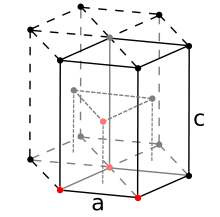
\includegraphics{hcp_edited.png}
		\end{figure}
		\subsection*{a) number of atoms in the cell}
			There are four lattice points that are shared between six unit cells, four that are shared between twelve and one atom in the middle of the unit cell
			$$\frac{4}{6}+\frac{4}{12}+1 = 2$$
		\subsection*{b) calculating the characteristic c/a ratio}
			The lattice point in the middle of the unit cell lies a distance $c/2$ above the bottom of the unit cell. This lattice point along with three other points on the bottom of the unit cell (indicated in red) creates a tetrahedron whose sides have length $a$. Finding c can now be done using trigonometry. First I find the distance between one corner of the tetrahedron to one of the adjacent sides.
			$$\cos(\pi /6) = \frac{a/2}{x} \implies x = \frac{a}{\sqrt{3}}$$
			This can now be put into the pythagorean theorem to find the relation between $c$ and $h$
			$$a^2 = (c/2)^2 + x^2$$
			$$c^2 = 4a^2-4x^2 = 4(a^2-\tfrac{a^2}{3})=8/3a^3$$
			$$\frac{c}{a}=\sqrt{\tfrac{8}{3}}$$
		\subsection*{c)}
			The packing density is the total volume of spheres in the unit cell divided by the volume of the unit cell. We already know there are only two full atoms in the unit cell and, since the distance between all atoms is $a$, the radius of these atoms is $r=a/2$. The volume of the unit cell is trivial to find once you realize that the area of the base, a parallellogram, is $A=\sqrt{3/4}a^2$. Our expression for $c$ also comes in handy.
			$$\frac{V_{spheres}}{V_{unit cell}}=\frac{ 2\tfrac{4}{3}\pi r^3 }{ \sqrt{{3}{4}} ca^2}$$
			$$= \frac{ \pi a^3 }{ 3\sqrt{\tfrac{8}{3}} \sqrt{\tfrac{3}{4}} a^3} $$
			$$=\frac{\sqrt{3}\sqrt{4}\pi}{3\sqrt{8}\sqrt{3}}$$
			$$=\frac{\pi}{3\sqrt{2}}\approx 76\%$$
		\subsection*{d)}
			This deviation resulting from some internal energy could mean that the material is not completely relaxed and is experiencing some strain.
	\newpage
	\section*{4: Reciprocal lattice}
		\begin{figure}[H]
			\centering
			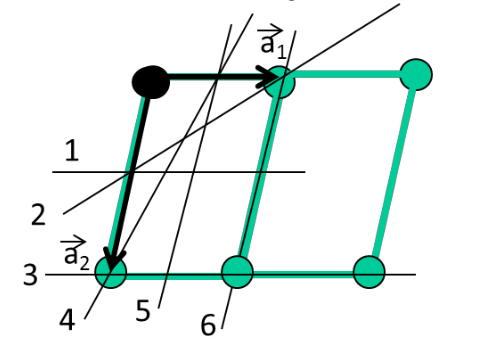
\includegraphics[width = 0.7\linewidth]{lattice.png}
		\end{figure}
		\subsection*{a)}
			The miller indinces of the planes are as follows:\\
			\begin{enumerate}
				\item $G_1 = (0,2,0)$
				\item $G_2 = (1,2,0)$
				\item $G_3 = (0,1,0)$
				\item $G_4 = (2,1,0)$
				\item $G_5 = (2,0,0)$
				\item $G_6 = (1,0,0)$
			\end{enumerate}
		\subsection*{b)}
			The formulas for the reciprocal lattice vectors are as follows:
			$$ \vb{b}_1 = 2\pi \frac{\vb{a}_2\vb{a}_3}{\vb{a}_1\cdot \vb{a}_2 \times \vb{a}_3}, \quad  \vb{b}_2 = 2\pi \frac{\vb{a}_3\vb{a}_2}{\vb{a}_2\cdot \vb{a}_3 \times \vb{a}_2}$$
			Since $\vb{a}_1\perp\vb{a}_3$ and $\vb{a}_2\perp\vb{a}_3$ the cross products gives vectors whose magnitude is the product of the magnitudes of vectors involved in the cross product and whose direction is perpendicular to the two vectors (direction decided by right hand rule). This makes it easy to immidiately draw $\vb{b}_1$ and $\vb{b}_2$.
			It can also be shown that $\frac{\vb{a}_1}{\vb{a}_2}=\frac{\vb{b}_2}{\vb{b}_1}$
			\begin{figure}[H]
				\centering
				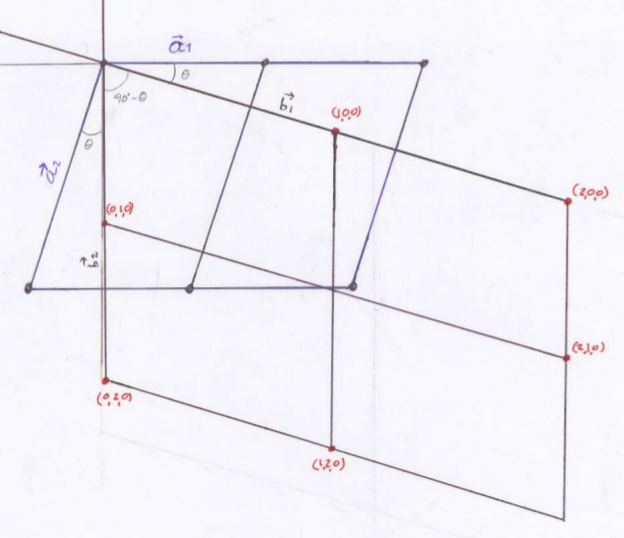
\includegraphics[width=0.7\linewidth]{reciprocal.png}
			\end{figure}
		\subsection*{c)}
			We know the definition of the change in wavevector (out minus in)
			$$\Delta\vb{k} = \vb{k}'-\vb{k}$$
			Also assume nearly completely elastic collisions with neglibile loss in kinetic energy
			$$\vb{k}^2 = \vb{k'}^2$$
			We start with the Laue condition
			\begin{align*}
				\Delta\vb{k} = \vb{G}\\
				\vb{k'}-\vb{k} = \vb{G}\\
				\vb{k'}^2=\vb{G}^2+2\vb{G}\vb{k}+\vb{k}^2\\
				\vb{G}^2 = 2\vb{G}{k}\\
				\frac{1}{2}G = \frac{\vb{G}\cdot\vb{k}}{G}\\
			\end{align*}
			The right side of this equation is the projection of k onto G, QED.
		\subsection*{d)}
			Since this requirement must hold for any of the reciprocal lattice points/reflections we can illustrate a 'forbidden' area where diffraction will not happen.
	\section*{7 Thermodynamics}
		\subsection*{a)}
			We want to find an expression for gibbs free energy, derive with respect to the number of vacancies $n$ and see where this is minimized. The entropy in gibbs free energy can be found by the binomial formula to check for number of microstates for $n$ vacancies in a crystal with $N$ lattice points. Stirlings approximation enables us get an estimation of the high factorials.
			\begin{align*}
				S = k\ln(\frac{N!}{n!(N-n)!})\\
				S \approx k(N\ln N -n\ln n - N\ln(N-n) + n\ln(N-n))
			\end{align*}
			The enthalpy can be exrepessed in terms of enthalpy per vacancy $H=n\Delta H_f$
			\begin{align*}
				G = H-TS\\
				\dv{G}{n}=\Delta H_f -T\dv{S}{n}\\
				=k(\ln(N-n)-\ln n\\
				=\Delta H_f-kT(\ln(N))-\ln n)\\
				=\Delta H_f + kT \ln(n/N)
			\end{align*}
			Finding the minimum gives
			\begin{align*}
				\dv{G}{n} = 0=\Delta H_f + kT \ln(n/N)\\
				n/N = \exp(-\frac{\Delta H_f}{kT})
			\end{align*}
		\subsection*{b)}
			Using the fact that $\Delta H_f =E_f+ \sigma V_f$ we get
			\begin{align*}
				C_v = n/N = \exp(-\frac{\Delta H_f}{kT})=\qty(-\frac{E_f+ \sigma V_f}{kT})
			\end{align*}
		\subsection*{c)}
			In chemistry the activation energy is the energy required for a reaction to take place. Even though the reaction may be exothermic and in that way favourable, it could take a lot of energy for the necessary parts to come together to make the reaction happen. Here, however, the activation energy is defined as the energy difference before and after a vacancy has been created. The activation volume is how much the volume changes after this vacancy is introduced. The volume might increase or decrease, depending on the crystal.
		\section{8 SiGe alloy}
			\subsection{a1)}
				By using the forumula and appropriate values we can calculate this directly
				\begin{align*}
					\sigma_0 = -2\mu\frac{\nu+1}{\nu-1}f_m(X)\\
					\sigma_0 = -2\times52GPa\frac{1.28}{-0.72}\times \frac{0.0418}{5}\\
					\sigma_0 \approx 1.546\times 10^9
				\end{align*}
			\subsection{b)}
				The vacancy concentration dependance of the diffusion coefficient can be taken to be proportional.
				Looking at the figure we can see that there is factor ten increase in the diffusion coefficient of the biaxially compressed lattice compared to the normal lattice. This should therefore also mean that there are ten times as many vacancies in this lattice
\end{document}